\ifspanish

\question  Considérese un sistema de comunicaciones en el que los símbolos ``$+1$'' ó ``$-1$'' se transmiten simultáneamente por dos canales ruidosos, tal y como se ilustra en la figura:
\begin{figure}[h]
\begin{center}
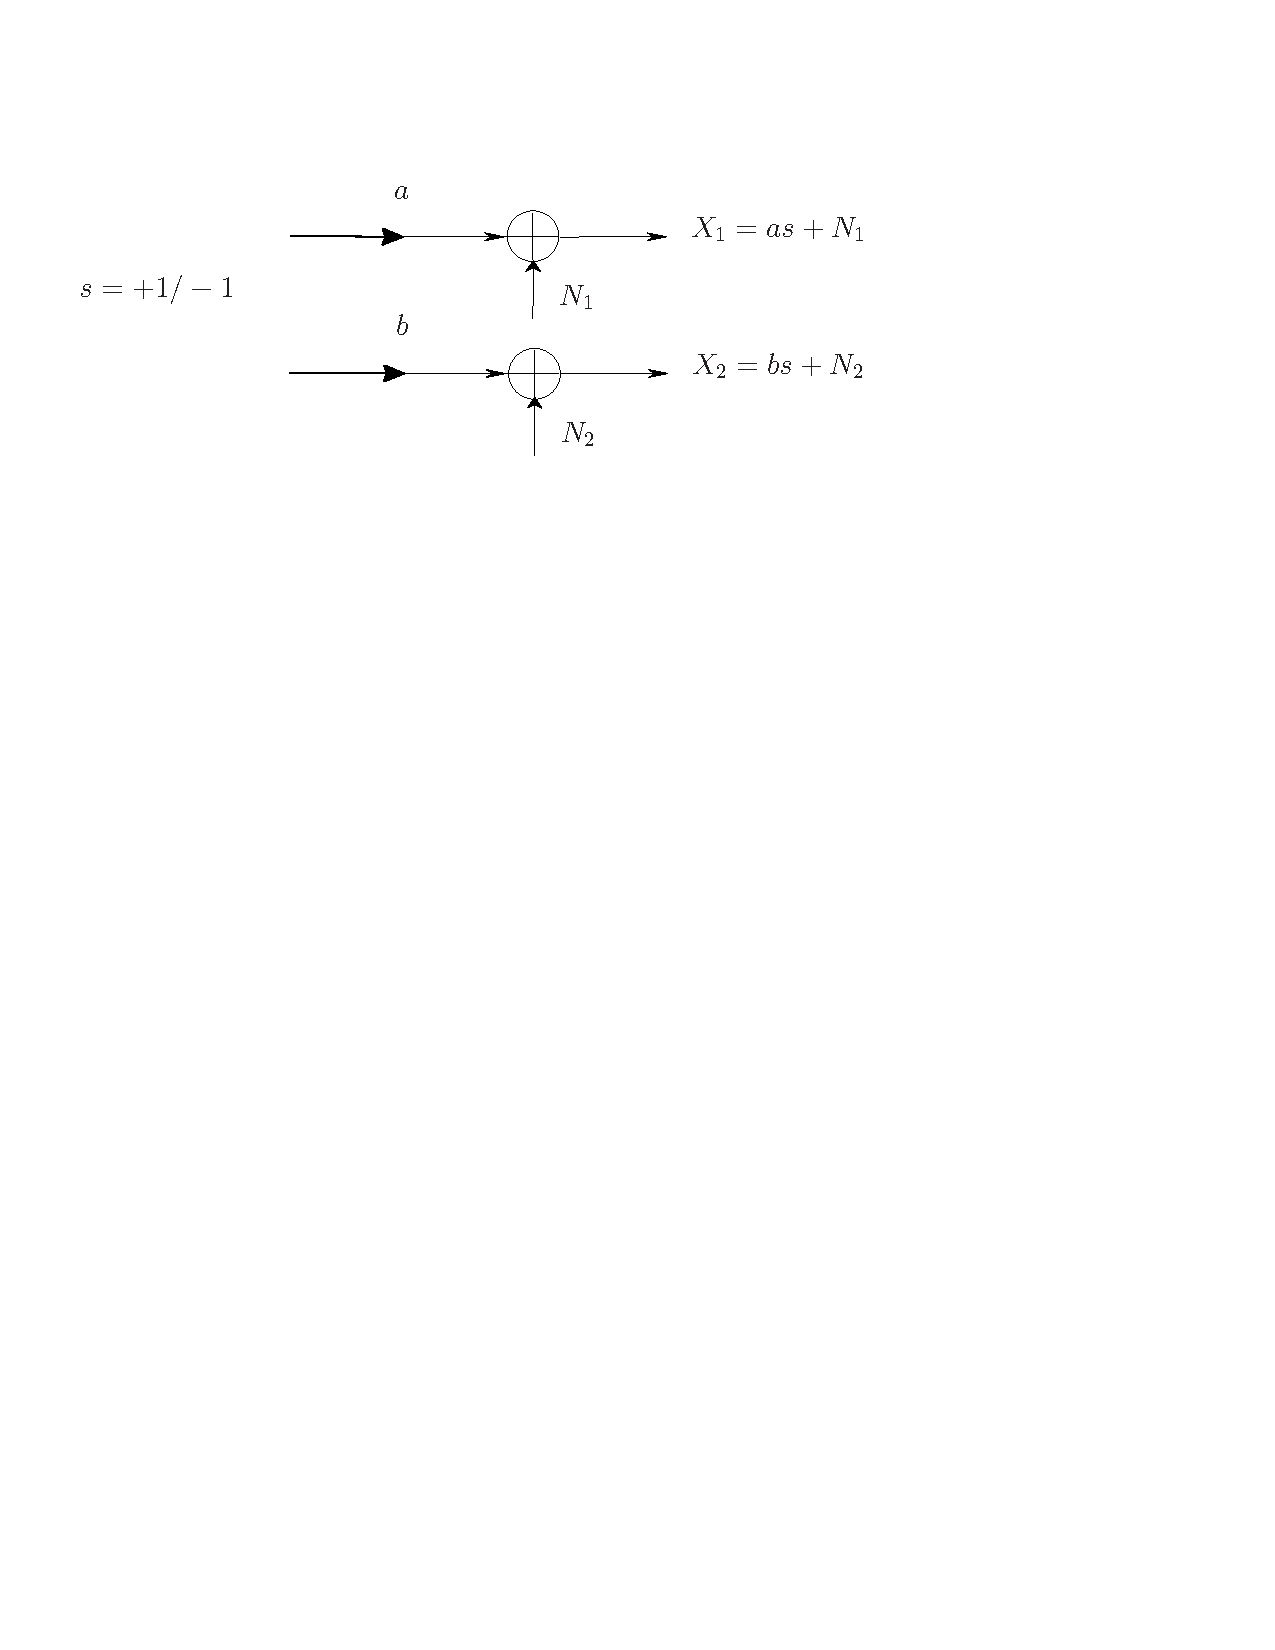
\includegraphics[width=12cm, trim=0cm 20.5cm 4cm 2.5cm]{Figuras/canal_gauss}
\end{center}
\end{figure}

siendo $a$ y $b$ dos constantes positivas desconocidas que caracterizan a los canales y $N_1$ y $N_2$ dos variables de ruido gaussiano caracterizados por
$$ \left( \begin{array}{c}  N_1 \\ N_2 \end{array}  \right) \sim G \left[ \left( \begin{array}{c}  0 \\ 0 \end{array}  \right), \left( \begin{array}{cc}  1 & \rho \\ \rho & 1 \end{array}  \right) \right].  $$
donde $|\rho|<1$. Se sabe, además, que las probabilidades de transmisión de ambos símbolos son iguales.
\begin{parts}
\part Si se desea construir un decisor para discriminar cuál fue el símbolo transmitido utilizando únicamente una de las dos observaciones disponibles, $X_1$ o $X_2$, indíquese cuál de las dos variables utilizaría, justificando su respuesta en función de los valores de las constantes.  Proporciónese la forma analítica del decisor ML correspondiente.
\part Obténgase el decisor binario de mínima probabilidad de error basado en la observación conjunta de $X_1$ y $X_2$, expresando el resultado como función de $a$, $b$ y $\rho$.  Simplifique la expresión de dicho decisor tanto como le sea posible.
\part Para $\rho = 0$, calcúlese la probabilidad de error del decisor dise\~{n}ado en b).  Exprese su resultado utilizando la función:
$$F(x) = 1- Q(x) = \int_{-\infty}^x \frac{1}{\sqrt{2\pi}} \exp{\left( - \frac{t^2}{2}\right) } \; dt$$

\end{parts}

\begin{solution}

\begin{parts}
\part $ \mbox{Si} \; a>b:  \quad  x_1 \dunodcero 0 \quad \quad  \quad  \quad \quad   \mbox{Si} \;  a<b: \quad  x_2 \dunodcero 0$
\part $(a - \rho b)x_1 + (b - \rho a)x_2 \dunodcero 0$
\part $\displaystyle  P_{\rm e}=F(-\sqrt{a^2+b^2})$ 
\end{parts}
 \end{solution}

\else

\question Consider a communication system in which one  of the symbols, ``$+1$'' or ``$-1$'', is simultaneously transmitted through two noisy channels, as illustrated in the figure:
\begin{figure}[h]
\begin{center}
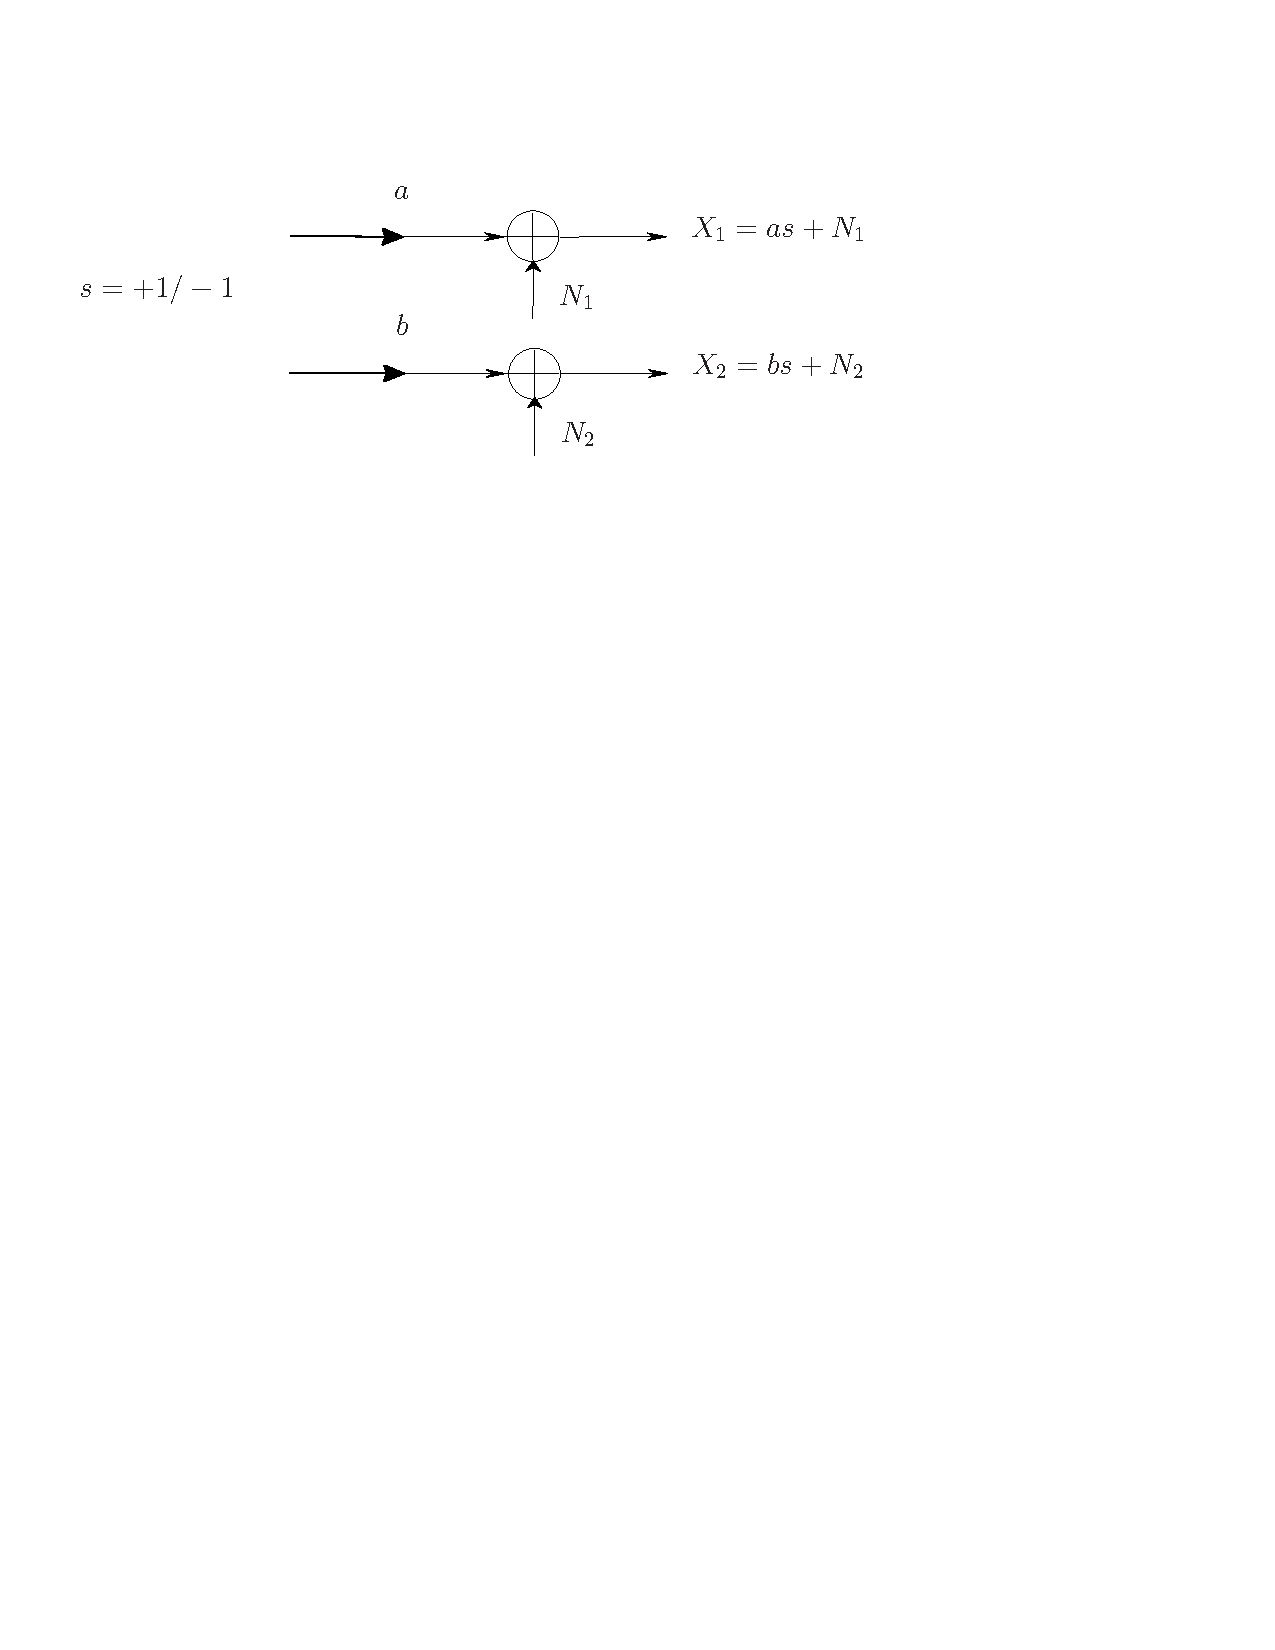
\includegraphics[width=12cm, trim=0cm 20.5cm 4cm 2.5cm]{Figuras/canal_gauss}
\end{center}
\end{figure}

with $a$ and $b$ being two unknown positive constants which characterize the channels, and where $N_1$ and $N_2$ are two Gaussian noises with joint pdf
$$ \left( \begin{array}{c}  N_1 \\ N_2 \end{array}  \right) \sim G \left[ \left( \begin{array}{c}  0 \\ 0 \end{array}  \right), \left( \begin{array}{cc}  1 & \rho \\ \rho & 1 \end{array}  \right) \right].  $$
It is also known that both symbols can be transmitted with equal {\em a priori} probabilities.
\begin{parts}
\part If we wish to design a decision maker for discriminating the transmitted symbol using just one of the two available observations, $X_1$ or $X_2$, indicate which of the two variables you would use, justifying your answer as a function of the values of constants $a$ and $b$.  Provide the analytical expression for the corresponding ML classifier.
\part Obtain now the binary classifier with a minimum probability of error, based on the joint observation of $X_1$ and $X_2$, expressing it as a function of $a$, $b$, and $\rho$. Simplify your expression as much as possible.
\part For $\rho = 0$, calculate the probability of error of the decision maker obtained in b). Express your result by means of function:
$$F(x) = 1- Q(x) = \int_{-\infty}^x \frac{1}{\sqrt{2\pi}} \exp{\left( - \frac{t^2}{2}\right) } \; dt$$

\end{parts}

\begin{solution}

\begin{parts}
\part $ \mbox{If} \; a>b:  \quad  x_1 \dunodcero 0 \quad \quad  \quad  \quad \quad   \mbox{If} \;  a<b: \quad  x_2 \dunodcero 0$
\part $(a - \rho b)x_1 + (b - \rho a)x_2 \dunodcero 0$
\part $ P_{\rm e}=F\left(-\displaystyle\sqrt{a^2 + b^2}\right)$ 
\end{parts}

\end{solution}

\fi